\begin{frame}{Modeling Outline}
Propagating a very dense pulse will require extra planning. A model for designing a UEM column needs:
	\begin{itemize}[<+->]
	    \item Generation dynamics
		\item Propagation dynamics
		\item Acceleration and gun effects
		\item Lenses and/or compressors	
		\item Apertures (?)
		\item Speed (multiple runs for optimization)
	\end{itemize}
No model existed that had all these features.
\end{frame}

\begin{frame}{Pulse Modeling}
	Analytic Gaussian (AG) model of Michalik and Sipe\footcite{michalik_analytic_2006}: 
	\begin{itemize}
		\item<2-> Self-similar Gaussian electron packet
		\item<3-> 6D (3 position \& 3 momentum) moment analysis
		\item<4-> Mulitdimensional Gaussian integral
		\item<5->[$\Rightarrow$] Reduces free-space propagation dynamics to six first order coupled differential equations!
	\end{itemize}
    While this model is the propagation engine of my model, alone it lacks:
    \begin{itemize}
      \item<6-> Electron-optical elements
      \item<7-> Realistic initial conditions
    \end{itemize}
\end{frame}

\begin{frame}{AG Model Extension\footcite{berger_semi-analytic_2010}}
\begin{columns}
  \begin{column}{0.54\linewidth}
    The extended AG model adds:
    \begin{itemize}
      \item Linear external forces
      \begin{itemize}
        \item<2-> Magnetic lenses
        \item<2-> RF Cavities
        \item<3-> Anode lensing ($E_{DC}$ by FEM)
      \end{itemize}
      \item<4-> Gaussian laser initial conditions (manuscript in prep.)
      \item<5-> Apertures (inc. pending dynamic lensing analysis)
    \end{itemize}
  \end{column}
  \begin{column}{0.4\linewidth}
    \begin{figure}
      \centering
      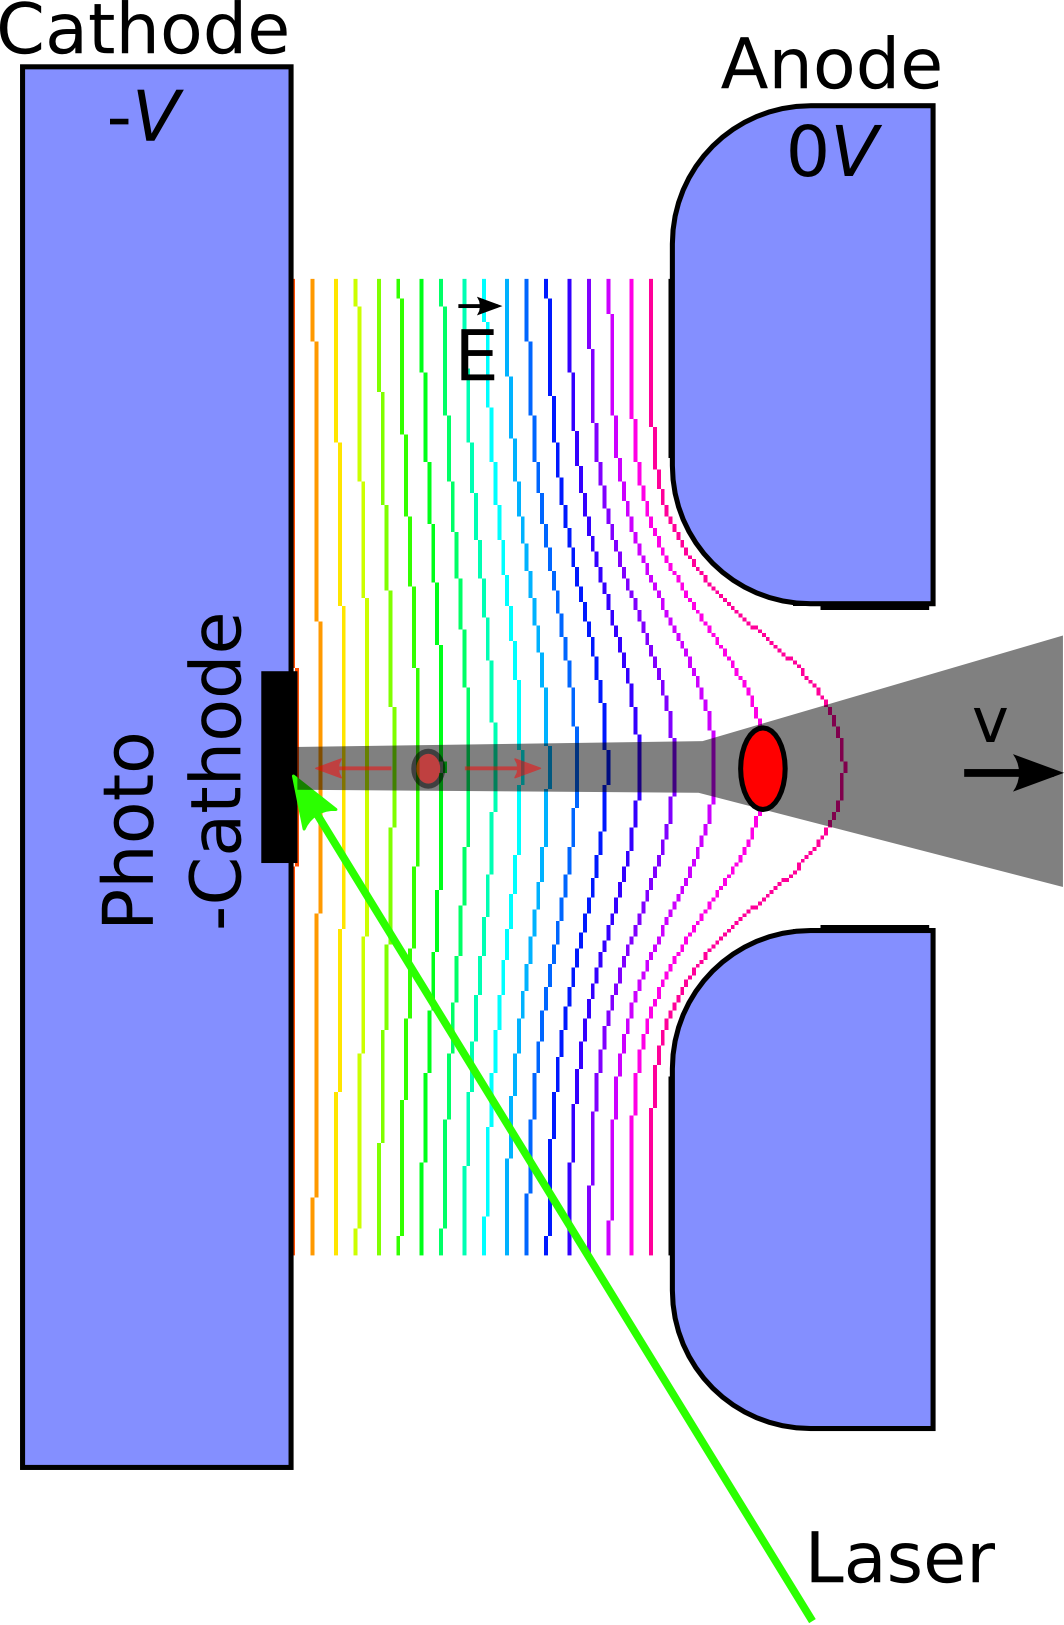
\includegraphics[width=0.5\linewidth]{acc_field}\\
      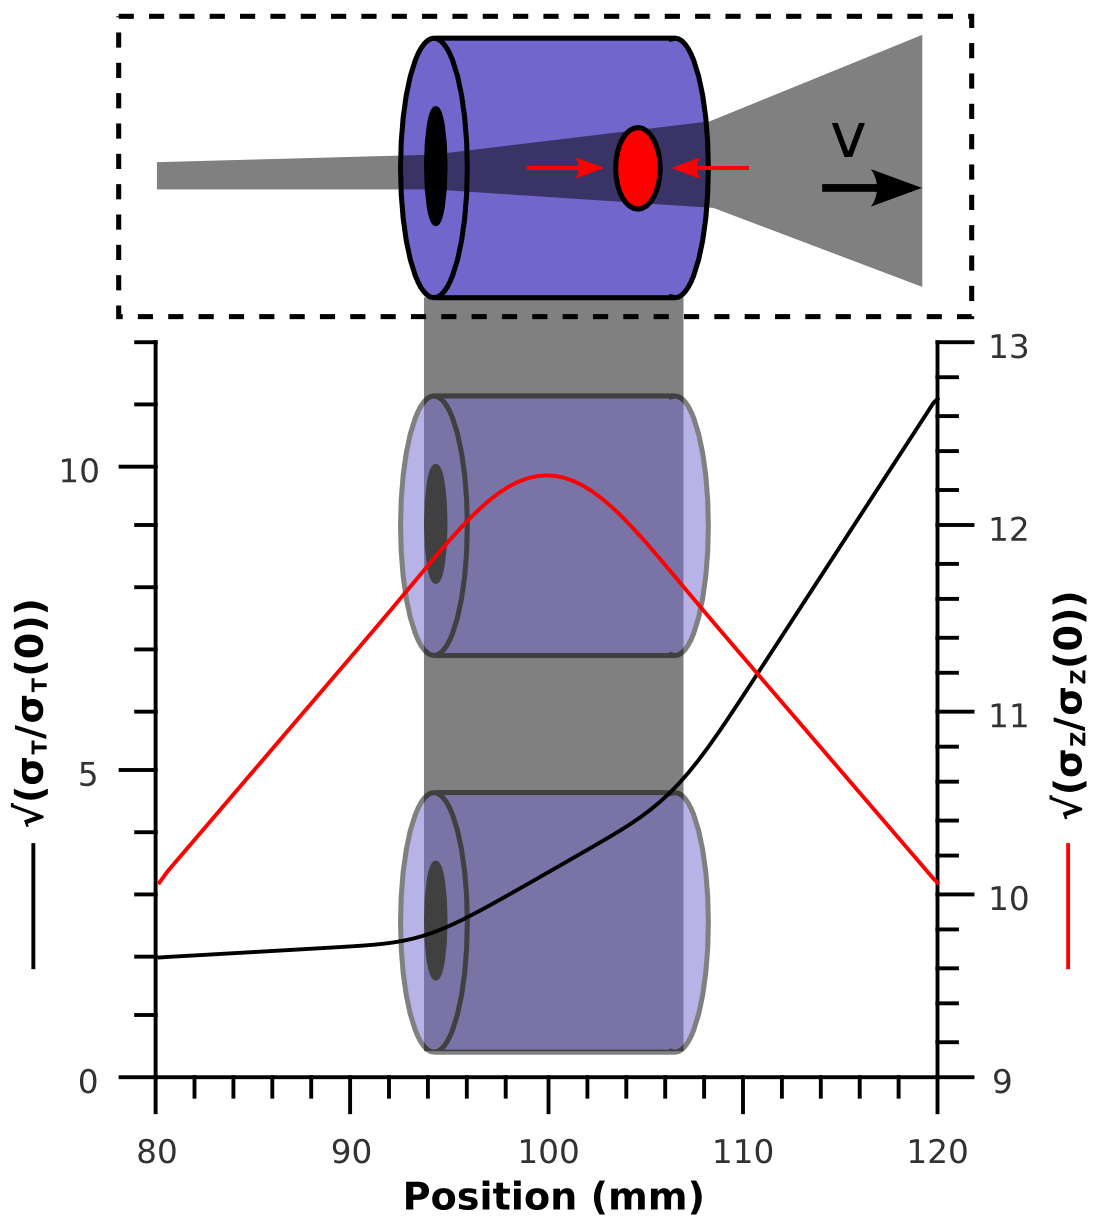
\includegraphics[width=0.5\linewidth]{RFCav}
    \end{figure}
  \end{column}
\end{columns}
\end{frame}

\begin{frame}{AG Model Example}
  \begin{center}
    %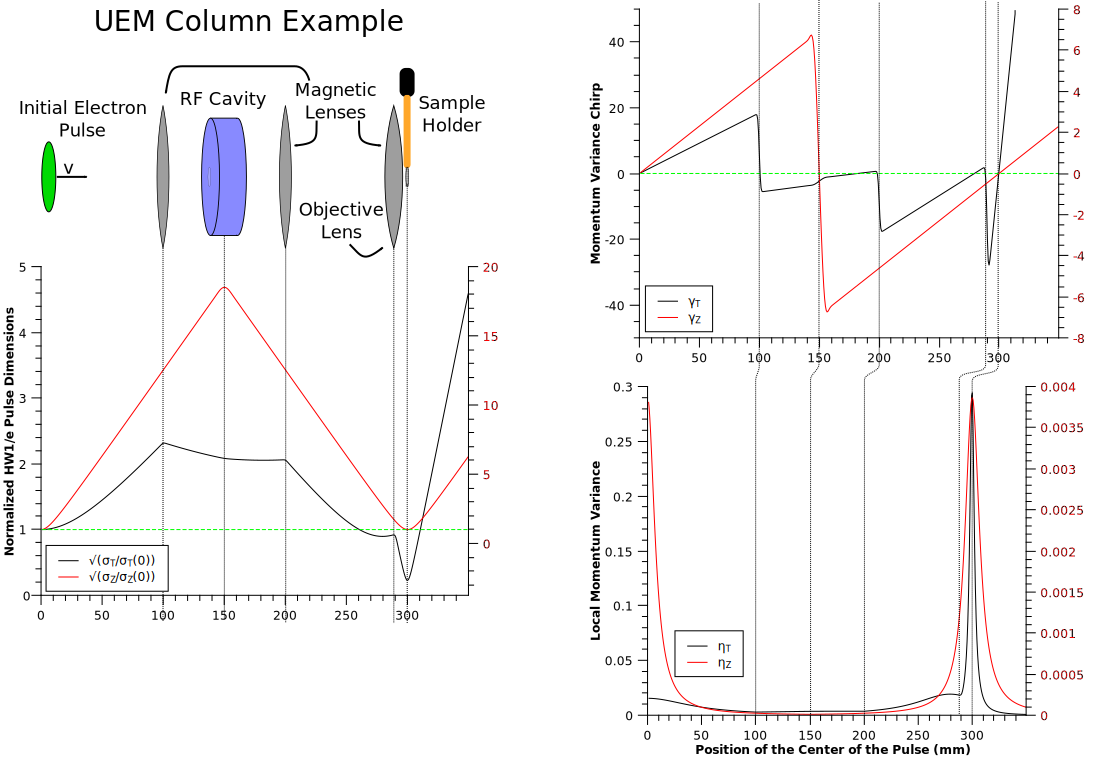
\includegraphics[width=0.7\linewidth]{Cooke_Column}
    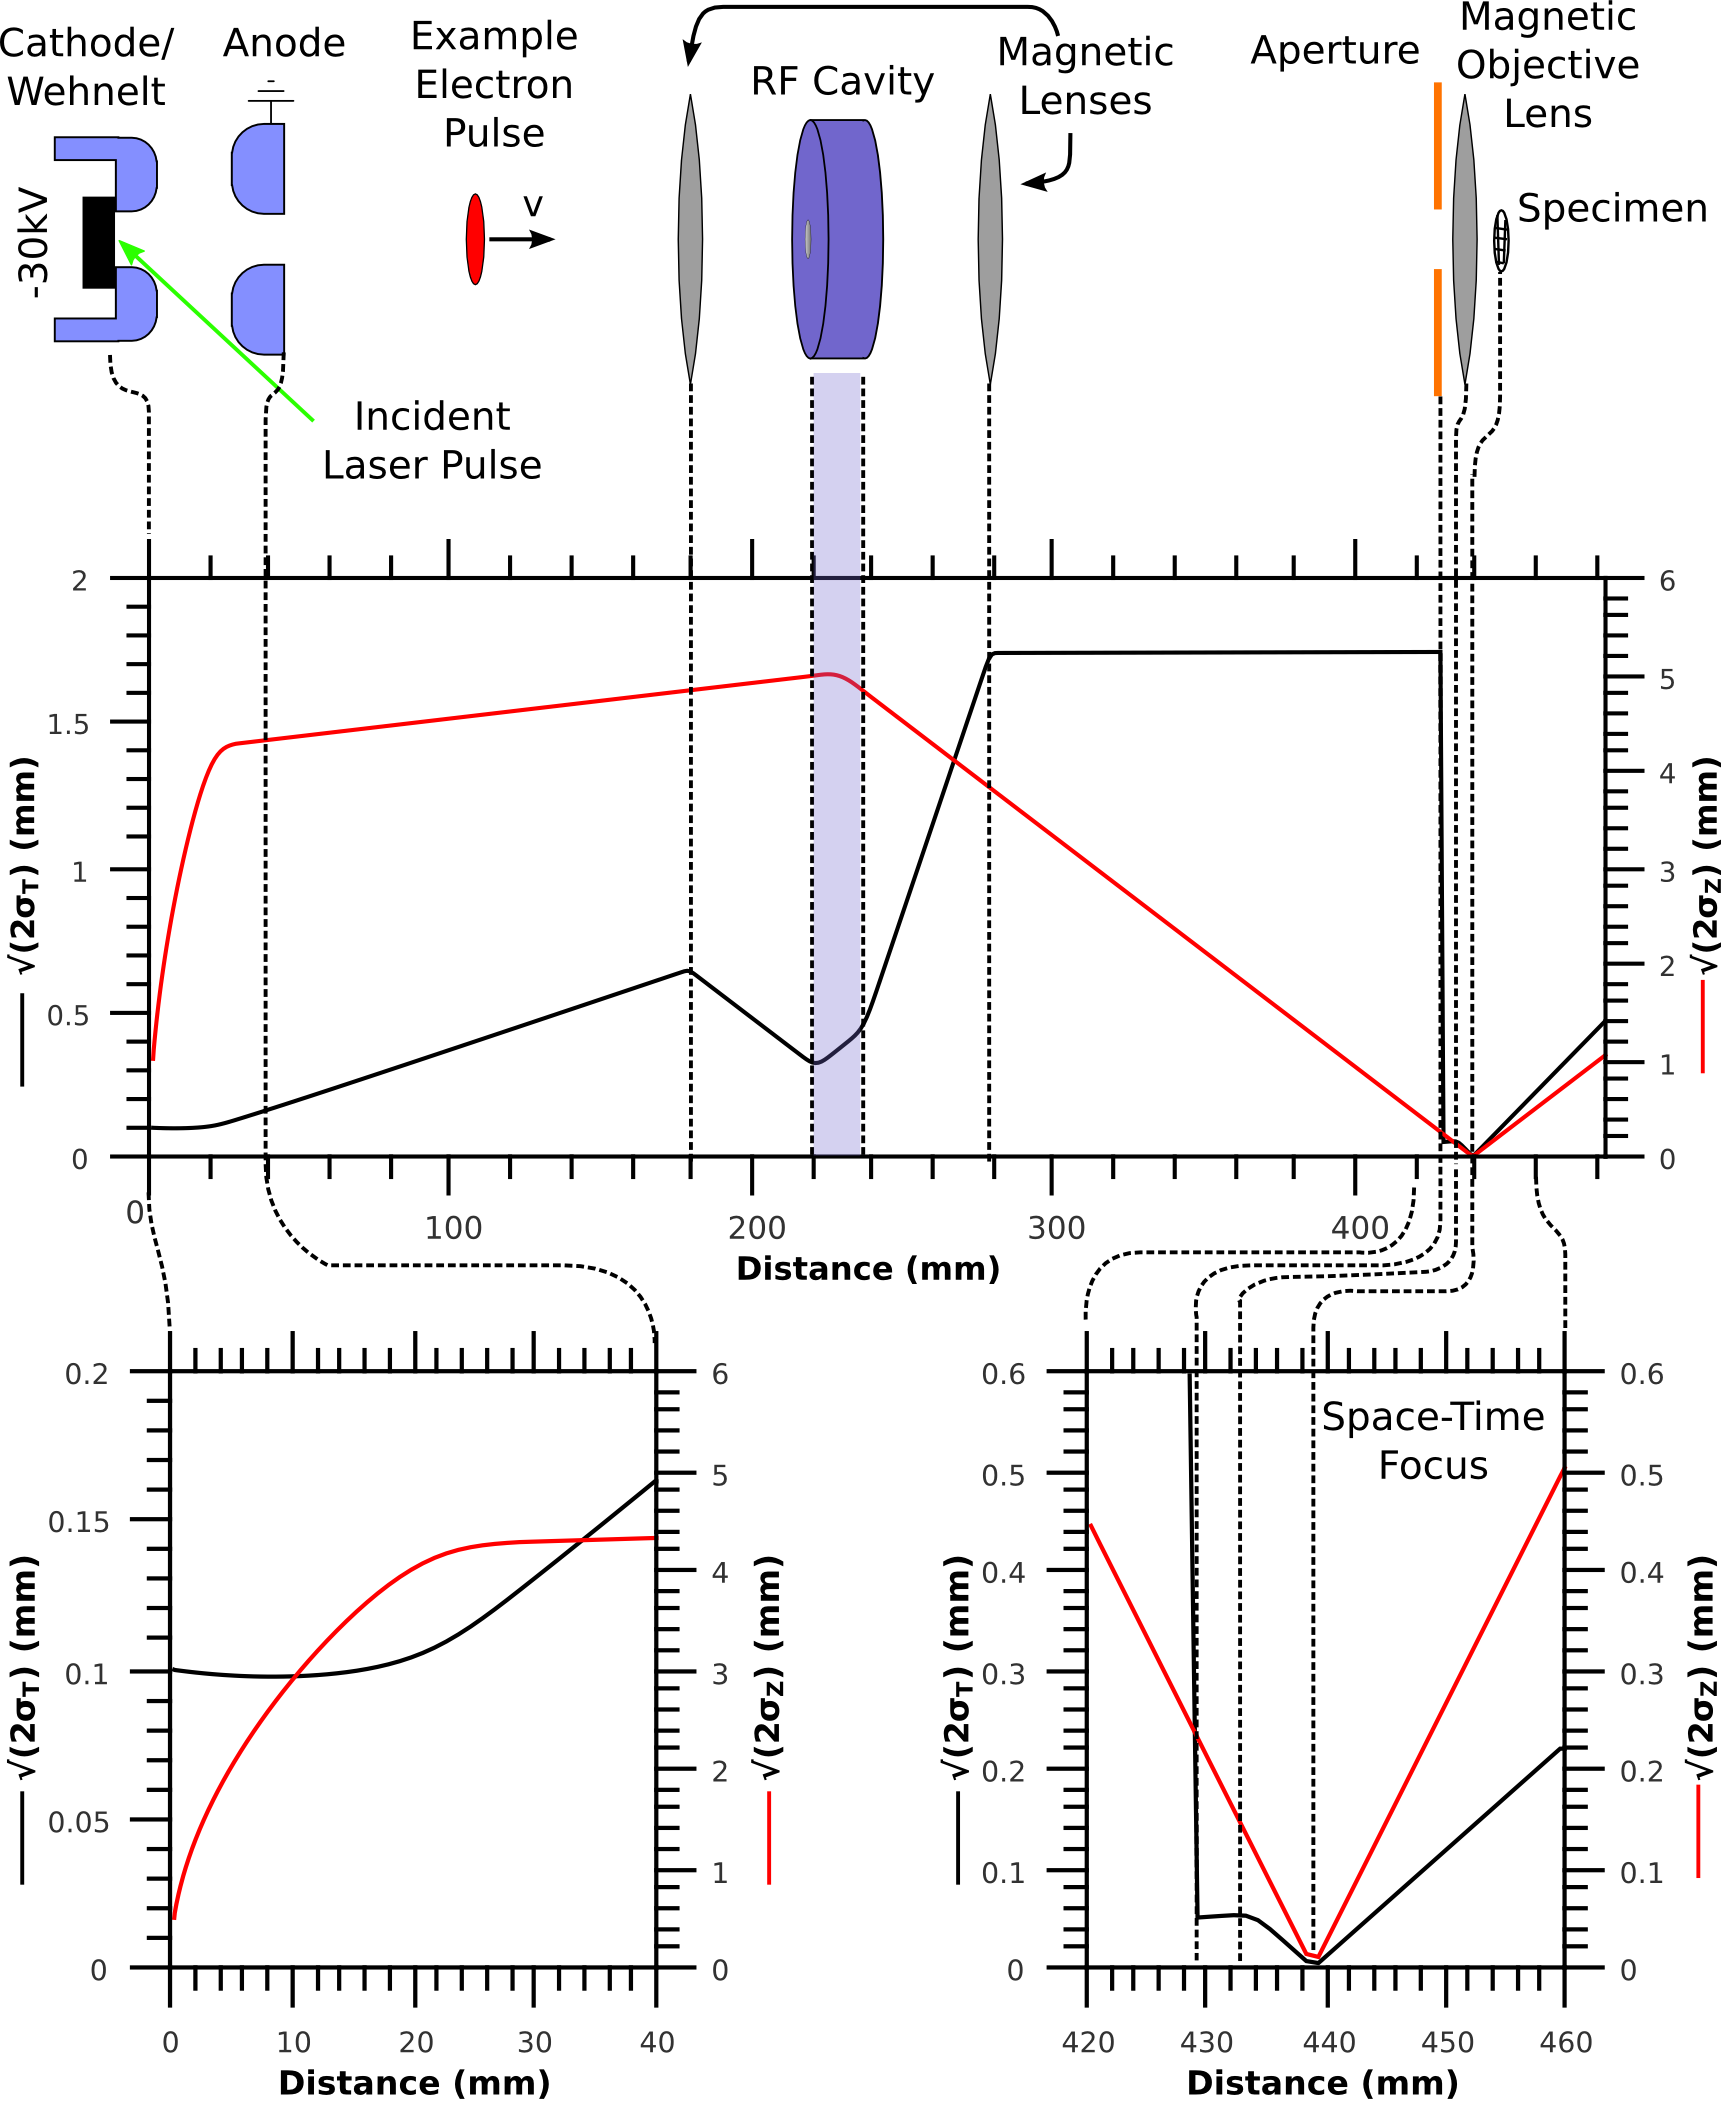
\includegraphics[width=0.5\linewidth]{Column}
  \end{center}
\end{frame}